% the sample slide is created with 16:9 aspect ratio
\documentclass[aspectratio=169]{beamer}

% remove the options if you do not want to have them
\usetheme[
	% background=images/background.jpg, % you can add your own background image
	logo=images/unsw-portrait.png,
	sidelogo=images/unsw-landscape.png,
]{unsw}
% uncomment to show notes. Works very nicely with dspdfviewer. You get something similar to PPT's presenter view.
\usepackage{pgfpages}
\usepackage{graphicx}
\usepackage{amsmath, amssymb, lmodern}
\graphicspath{{images/}}
%\setbeameroption{show notes on second screen}

% information for the title page
\author{Isitha Subasinghe}
\title{Verification of programs in the presence of shared memory under weak memory consistency}
\subtitle{Linear Types to the rescue}
\institute{School of Computer Science and Engineering}
\date{\today}

\begin{document}
	% use plain option to remove the page number from the title slide
	\begin{frame}[plain]
		\titlepage
	\end{frame}
	
	\begin{frame}{Introduction}
    \framesubtitle{The seL4 core platform and sDDF}  
    The seL4 core platform is a lightweight operating system intended to replace CAmkES.
    This component was verified as of the last NCSC delivery phase. 
    \\ \vspace{20pt}
    Building on top of this exists the sDDF which provides a mechanism for writing device drivers. This component is unverified but the intention is to eventually verify a network multiplexer which builds upon the sDDF. 
	\end{frame}

  \begin{frame}{What does the multiplexer look like?}
    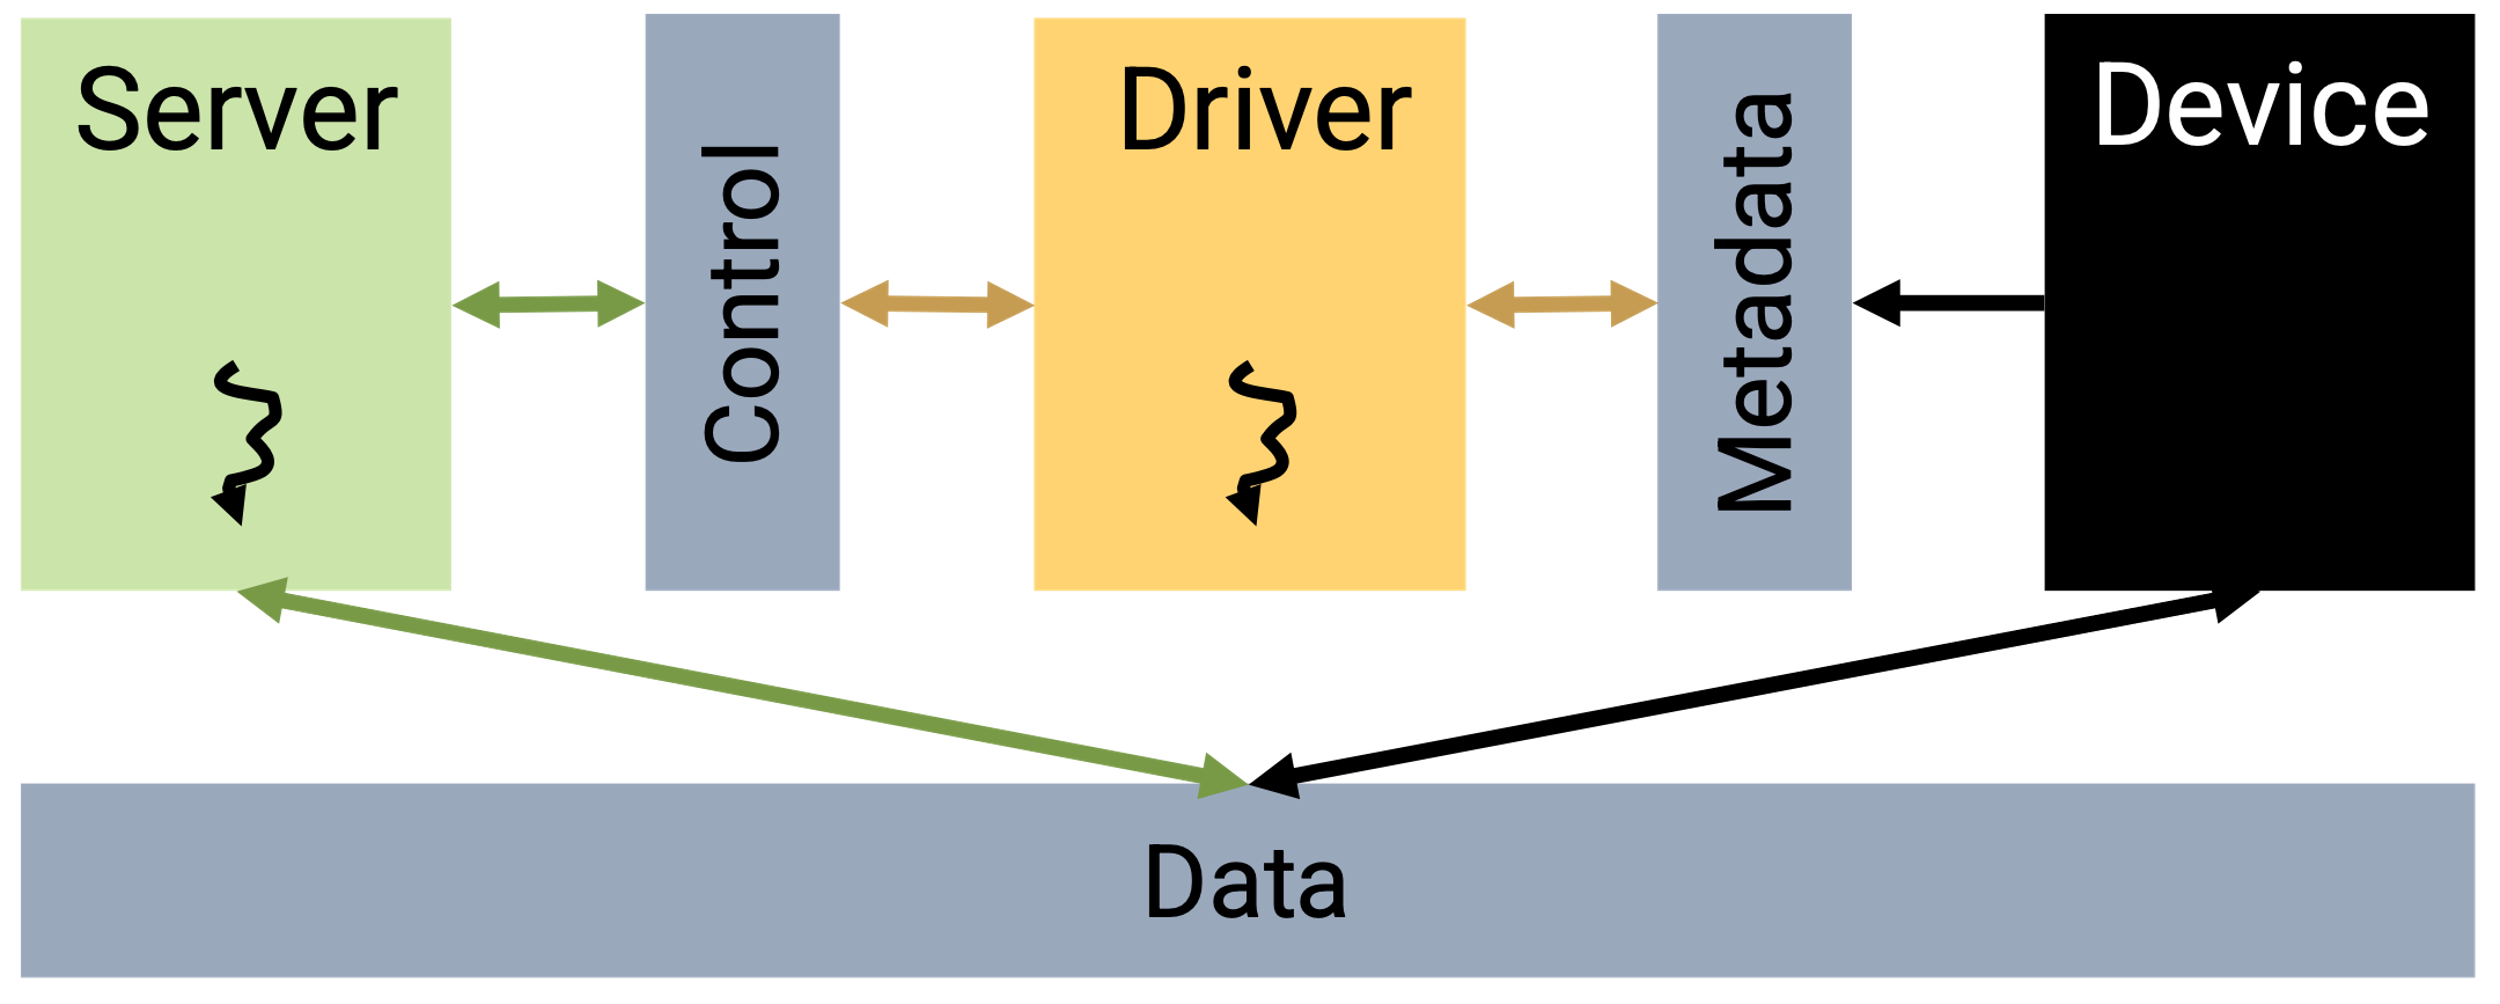
\includegraphics[width=\textwidth]{sddf_arch} 
  \end{frame}

  \begin{frame}{What does the multiplexer look like?}
    \begin{itemize}
      \item Shared memory to transfer data (buffers) from the NIC.
      \item Single producer, single consumer ring buffer between the various components to transfer said data (note that the ring-buffer itself is shared memory).
    \end{itemize}
  \end{frame}

  \begin{frame}{Tuch's model of memory}
    Tuch's memory model initially establishes memory as an array of bytes, but then attempts to lift these into 
    types that is easier to reason about. For context, proofs relating to this memory model was to be reasoned in Isabelle, this means that the 
    byte level granuality is massively inconvinient. To this extent, Tuch's model makes the use of multiple typed heaps, this has the added advantage of being 
    able to reason about intra-type aliasing. Tuch states that the use of separation logic is needed handle inter-type aliasing. 
  \end{frame}

  \begin{frame}{Hypothesis}
    \framesubtitle{Tuch's memory model doesn't buy us much}
    While Tuch's memory model makes sense in the context of Isabelle proofs, it is a reasonable question to ask 
    if encoding the tracking of each address and its type and support for multiple typed heaps is worth the effort when we are going to reason about all our variables as bit vectors anyway. 
  \end{frame}

  \begin{frame}{Alternative model}
    What may be the better solution with regards to SMT solvers is to treat memory like an array of indexed bit vectors. 
    This is easy to encode in SMT using QF\_ABV alone.
    \\ \vspace{20pt}
    A question that naturally arises is that of how to model structs in this view of memory. 
    Michael Norrish's C parser solves this for us as all structs are scalarised.
    This reinforces the previous point with regards to Tuch's memory model, bit vectors are all we need!
  \end{frame}
  
  \begin{frame}{How do we model pointer operations?}
    \begin{itemize}
      \item Logical model 
      \item Concrete model 
    \end{itemize}
  \end{frame}

  \begin{frame}{Logical model of pointers}
    The simplest way to model pointers is to encode them as consisting of a base address and an offset. 
    This model gets us far but fails to accomadate integer to pointer casts as information is lost during this process. 
    \begin{alertblock}{MIRI}
      In fact, MIRI, an interpreter for the Mid-level Intermediate Representation used to catch undefined behaviour is not able to handle integer to pointer casts and remain sound.
    \end{alertblock}
  \end{frame}
  
  \begin{frame}{Logical model of pointers}
    \framesubtitle{Integer to pointer casts}
    Well unfortunately this isn't good enough for general C programs. It turns out those pesky C programmers do insane things such as 
    converting integers to pointers and back. There are naive solutions to tackle this problem, but unfortunately they come with serious downsides. 
    \begin{itemize}
      \item View all integers as pointers
      \item An analysis pass to determine which integer variables needed to be reasoned about as pointers. 
    \end{itemize}
  \end{frame}

  \begin{frame}{Concrete model of memory}
    Alternatively we can reason about memory as an array of bytes (depending on granularity desired).
    This solves the big problems when it comes to the logical model but now requires quantifiers. 
    This means that QF\_ABV might not be enough. 
  \end{frame}

  \begin{frame}{Do we have to compromise?}
    Neither of these memory models are without their downsides and it has rightly prompted researchers to ask the question ``Is there a better alternative?''. 
    Unfortunately, the answer to that question is only a maybe so far. Work done by Kang and others show that it is possible to interleave these two models, that is, 
    using the more encoding efficient representation (logical) until a cast to an integer occurs. 
    \\ \vspace{20pt}
    The issue with this approach is it's complexity, essentially relying on two models and a transition phase to be encoded correctly, furthermore in the worst case, 
    we might degrade into a concrete model of memory. 
  \end{frame}

  \begin{frame}{Do we have to compromise?}
    Perhaps we can get away with some smart encoding of what the quantifiers encode?
    Assume we would like to have the following pointer validity condition: $\forall |i: int, p: addr| i < 10 \wedge i \geq 0 ==> pvalid(p+i)$
    We can encode this in SMT by declaring an integer i exists and then assuming the correct range, this essentially boils away the quantifier. 
  \end{frame}

  \begin{frame}{Aliasing}
    One problem that occurs when encoding memory is the question of aliasing. 
    If we have aliased memory, then we lose the certainty that any pointer's underlying memory did not change. 
    One easy solution is to have linearly typed memory regions, ownership is passed from function to function based on usage. 
    This is what Verus does in the form of linear ghost permissions to enable support for raw heap pointers. 
    Verus introduces a ``PPtr$<$T$>$'' which is called a permission pointer which is associated with a ``PermData$<$T$>$''. 
    One can think of PermData as a capability to do pointer operations on PPtr.
  \end{frame}

  \begin{frame}{Is this powerful enough to handle a ring buffer?}
    Yes! Verus shows that linear ghost permissions are powerful enough to handle a FIFO ring buffer. 
  \end{frame}

  \begin{frame}{Handling DMA cache-incoherent memory}
    Direct Memory Access that a device driver entirely bypasses the CPU and as a result. 
    The requirements for DMA memory is fairly easy to verify. What is harder is knowing which memory itself is DMA, this is easy by inspection but not automatically.
    Given we can do this, we need to ensure prior to a read from DMA memory, a cache invalidation is performed and prior to a write that a cache flush is performed.
  \end{frame}
  
  \begin{frame}{Verification of the shared ring buffer}
    \framesubtitle{Hypothesis}
    There exists an ordering relationship between the memory consistency in the enqueue and dequeue operations. 
  \end{frame}

  \begin{frame}{Verification of the shared ring buffer}
    \framesubtitle{dequeue}
    Let's look at the dequeue implementation. 
  \end{frame}

  \begin{frame}{Verification of buffers in the presence of concurrency}
    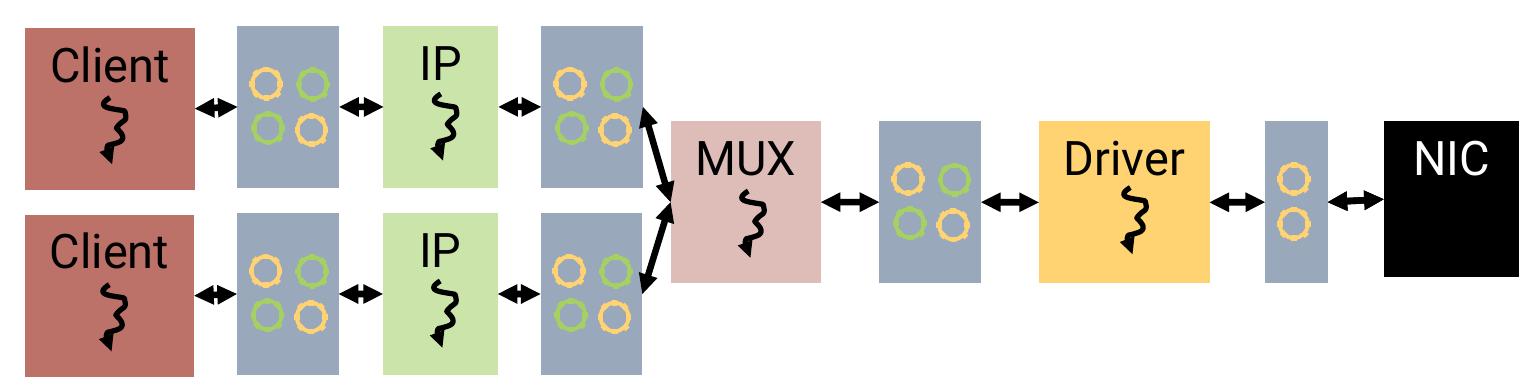
\includegraphics[width=\textwidth]{sddf_detail} 
  \end{frame}

  \begin{frame}{Verification of buffers in the presence of concurrency}
    \framesubtitle{Linearly typed buffers}
    We want to prove globally that a single buffer is ever ``owned'' by one component, 
    we can make an informal argument that 
  \end{frame}

  \begin{frame}{Conclusion}
    Linear Types are great!
  \end{frame}

  \begin{frame}[allowframebreaks]{References}
    \bibliographystyle{amsalpha}
    \nocite{*}
    \bibliography{ref}
  \end{frame}
\end{document}
